\documentclass{article}
\usepackage[utf8]{inputenc}
\usepackage{graphicx}
% we use paracol to display breakable two columns
\usepackage{paracol}
% define page styles using geometry
\usepackage[a4paper]{geometry}

% remove all possible margins
\geometry{top=1cm, bottom=1cm, left=1cm, right=1cm}

% indentation is zero
\setlength{\parindent}{0mm}

% include the fontawesome icon set
\usepackage{fontawesome}

\usepackage{enumitem}
\usepackage{ragged2e}
%----------------------------------------------------------------------------------------
%	FONT BASICS
%----------------------------------------------------------------------------------------

% some tex-live fonts - choose your own

\usepackage[defaultsans]{droidsans}
%\usepackage[default]{comfortaa}
%\usepackage{cmbright}
% \usepackage[default]{raleway}
%\usepackage{fetamont}
%\usepackage[default]{gillius}
%\usepackage[light,math]{iwona}
%\usepackage[thin]{roboto} 

% set font default
\renewcommand*\familydefault{\sfdefault} 	
\usepackage[T1]{fontenc}
\usepackage{moresize}
%----------------------------------------------------------------------------------------
%	TABLE /ARRAY DEFINITIONS

% extended aligning of tabular cells
\usepackage{array}

% custom column right-align with fixed width
% use like p{size} but via x{size}
\newcolumntype{x}[1]{%
>{\raggedleft\hspace{0pt}}p{#1}}%
\usepackage{xcolor}
% light color
\definecolor{darkcol}{HTML}
{A4330D}%<{type: "reference", id: "color"}>

\usepackage{fancyhdr}

\renewcommand*\headrulewidth{0pt}
\newcommand{\sidebarsection}[1]{
    \large\textcolor{darkcol}{\textbf{#1}}
}
\newcommand{\recipesection}[1]{
    \LARGE\textcolor{darkcol}{\textbf{#1}}
}
\newcommand{\preparationitem}[1]{
    \normalsize\item{#1}
}
\newcommand{\recipetext}[1]{
    \textcolor{darkcol}{#1}
}
\newcommand{\ingredientitem}[1]{
    \vspace{3pt}
    \normalsize\emph{#1}
    \vspace{3pt}
}
\begin{document}
\pagenumbering{gobble}
\columnratio{0.76}
\setlength{\columnsep}{2.2em}
\setlength{\columnseprule}{4pt}
\colseprulecolor{darkcol}
\begin{paracol}{2}
\begin{leftcolumn}

%<{type: "group", description: "Receptinformatie"}
\begin{center}
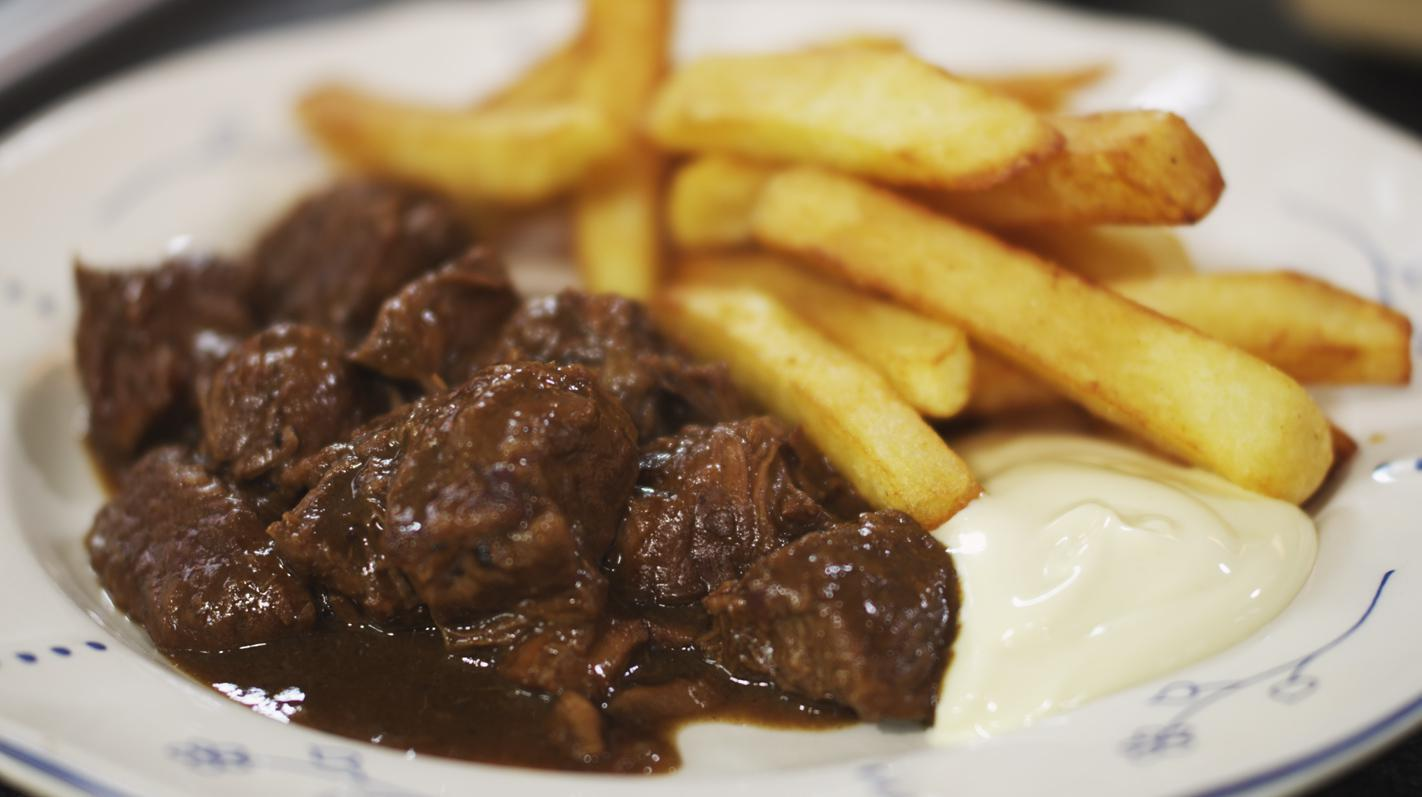
\includegraphics[width=\linewidth]{frietstoofvlees.jpg}%<{description: "Foto", type: "crop", aspect: 2}>
\end{center}
\recipesection{Friet stoofvlees} %<{description: "Titel recept", type: "text"}>
\vspace{0pt}
\\
\textcolor{darkcol}{\normalsize\faClockO\recipetext
{3u} %<{description: "Bereidingstijd", type: "text"}>
}
\textcolor{darkcol}{\normalsize\faUser\recipetext
{4 personen} %<{description: "Aantal porties", type: "text"}>
}
\textcolor{darkcol}{
\normalsize\faNewspaperO\recipetext{Dagelijksekost} %<{description: "Bron van het recept (optioneel)", type: "text", deleteOnEmpty: true}>
}
%>
\vspace{5pt}
\begin{enumerate}[wide, labelwidth=!, labelindent=0pt]
    %<{description: "Bereiding", type: "list", deleteOnEmpty: true}
        \preparationitem{Pel de uien en snipper ze in niet al te fijne stukjes.} %<{description: "Step", type: "textblock", injectBrackets: true}>
        
        \preparationitem{Verhit een ruime stoofpot en smelt er een klontje boter in. Stoof daarin de uien op een matig vuur. Laat de uien niet bruin bakken.}
        \preparationitem{Verhit een braadpan op een matig vuur en smelt er een klontje boter in.}
        \preparationitem{Schroei de stukken vlees in de braadpan tot ze een goudbruin kleurtje hebben. Kruid het vlees tijdens het bakken met wat peper van de molen en een snuifje zout.}
        \preparationitem{Doe de stukjes vlees in de stoofpot met uien. Hou de braadpan met aanbaksels bij en schenk daarin het bier. Roer alle aanbaksels van het vlees los terwijl het bier aan de kook gebracht wordt (deglaceren). Zodra het bier kookt, giet je het in de stoofpot}
        \preparationitem{Bind enkele blaadjes laurier en een paar takjes verse tijm samen met een eindje keukentouw. Laat het kruidentuiltje meestoven in de pot.}
        \preparationitem{Voeg de kruidnagel toe en de Loonse (of Luikse) appel-perenstroop.}
        \preparationitem{Besmeer het bruin brood royaal met (scherpe) mosterd. Leg de boterham in de pot, met de besmeerde zijde naar onder.}
        \preparationitem{Laat het stoofvlees anderhalf tot drie uur lang sudderen op een zacht vuur. Het deksel hoeft niet op de pot. De kooktijd is afhankelijk van de kwaliteit van het vlees. Roer af en toe eens in de pot en controleer tussendoor of het vlees voldoende gaar is. Pas zodra de stoofvleessaus de gewenste dikte heeft, plaats je het deksel op de stoofpot.}
        \preparationitem{Werk het stoofvlees af met een klein scheutje natuurazijn en roer alles om. Proef en voeg naar smaak nog wat peper van de molen toe en een snuifje zout.}
        \preparationitem{Schil de aardappelen en snij ze met de hand in gelijkvormige frieten. Was de frieten niet, want dan spoel je het zetmeel eraf. (tip Een ideale Belgische friet is 1,3 cm dik)}
        \preparationitem{Verhit het frietvet op 140°C. Bak de frietjes een eerste keer, maar laat ze nog niet kleuren. Laat de frietjes koud worden in een schaaltje met wat keukenpapier.}
        \preparationitem{Verhit het frietvet vervolgens tot 180°C. Bak de koude frieten nu goudbruin en knapperig. Giet de frieten opnieuw in een schaal met wat keukenpapier, zodat ze even kunnen uitlekken. Strooi er naar smaak wat zout over.}
        \preparationitem{Eet smakelijk!}
    %>

\end{enumerate}
\end{leftcolumn}

\begin{rightcolumn}

\sidebarsection{Ingrediënten} \\ \\
%<{description: "Lijst van ingrediënten", type: "list", deleteOnEmpty: true}
\ingredientitem{2 grote uien}\\ %<{description: "Ingrediënt", type: "text"}>
\ingredientitem{klontjes boter}\\
\ingredientitem{1kg rundsvlees}\\
\ingredientitem{peper en zout}\\
\ingredientitem{2 flesjes bruin bier bv. Sint Bernardus abt 12}\\
\ingredientitem{2 blaadjes laurier}\\
\ingredientitem{2 takjes tijm}\\
\ingredientitem{1 kruidnagel}\\
\ingredientitem{2 eetlepels Luikse stroop (appel of peer)}\\
\ingredientitem{2 eetlepels mosterd}\\
\ingredientitem{scheutjes natuurazijn}\\
\ingredientitem{1kg (loskokende) aardappelen}\\
\ingredientitem{mayonaise}\\
%>

\newcommand{\hide}[1]
{}

\hide{
    %<{type: "color", description: "Kies je eigen kleur (optioneel)", initialColor: "A4330D", id: "color"}>
}

\end{rightcolumn}
\clearpage
\end{paracol}
\end{document}
